\section{Introduction}\label{sec:intro}

\begin{figure*}[t]
\centering
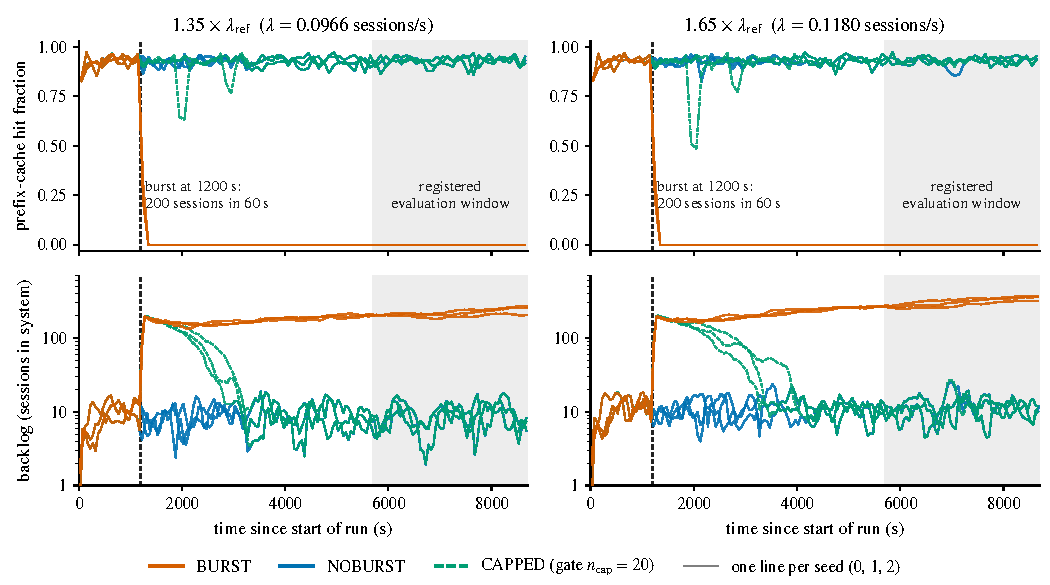
\includegraphics[width=\textwidth]{figs/fig1_e2_timeseries.pdf}
\caption{The stampede on SGLang: the registered paired test E2 at nominal rates of 1.35~$\lref$ (left) and 1.65~$\lref$ (right),
$\lref=0.0715$\sps, the all-miss session rate measured with the radix cache disabled; one A100, a 300k-token KV pool. Top: hit
fraction (turns with more than half of the prompt cached) in 100\,s windows. Bottom: sessions in the system (log scale), including
those in tool calls. One thin line per seed and arm. Dashed: a burst of 200 sessions at 1200\,s. Shaded: the registered evaluation
window. Without the burst (NOBURST) and with a client-side session cap (CAPPED) the engine stays good; after it (BURST), every turn
misses to the end of the run.}\label{fig:e2}
\end{figure*}

An LLM agent that calls tools sends its serving engine sessions of many turns: each prompt is the previous context plus the
output of the tool just run. Prefix caching keeps the key--value (KV) state of the previous turn, so a follow-up turn whose prefix
is still cached prefills only its new tokens~\citep{zheng2024sglang}. In our workload a hit prefills 551 tokens and a miss about
11{,}100, and a session's prefill work with every turn missing is about 16 times that with every follow-up hitting. The cached KV
belongs to sessions that sit idle in tool calls, and admitting waiting work evicts it. A burst of new sessions can therefore tip
the engine into a state in which every turn misses, the queue grows, the gap between a session's turns grows with it, and idle KV
is evicted before its owner returns. Fig.~\ref{fig:e2} shows this stampede on SGLang: at loads that the engine carried from empty,
a burst of 200 sessions left it at zero hits for the remaining 7500\,s.

\paragraph{What is not ours.} The phenomenon, its sustaining loop and a fluid model of its window are not new. Concurrently with
and independently of this work, Lu et al.\ showed on prefill--decode disaggregated SGLang with real agent traces that a finite surge
leaves the engine persistently degraded at a base load it previously sustained, identified the population--cache feedback that
sustains the failure, and modelled the vulnerable window with a fluid population balance and an empirical hit-rate
curve~\citep{lu2026cachetrap}. Their paper appeared first. The registered stampede and recovery experiments of \S\ref{sec:stampede}
were designed, registered and run between 21 October and 1 November 2026, before it appeared (Appendix~\ref{app:reuse}); the theory
of \S\ref{sec:trap}, the blind tests of \S\ref{sec:validation} and~\S\ref{sec:control} (registered on 2026-11-05) and MIRROR came
% MIRROR: drop "and MIRROR" if MIRROR is not reported
afterwards, and the trap-state predictions were made with Lu et al.'s paper in hand. The collapse is Denning's
thrashing~\citep{denning1968thrashing}, a bad state that a feedback loop sustains after its trigger is a metastable
failure~\citep{bronson2021metastable,huang2022metastable}, and metastability from a unimodal throughput curve, with bounded admission
as the cure, is classical~\citep{kleinrock1975aloha,carleial1975bistable,nelson1987stochastic}.

\paragraph{The question.} This paper asks what the trapped state \emph{is}. Quasi-static models treat it as the falling branch
of a throughput curve, $\dot n=\lambda-\mu(n)$; read literally in congestion, sessions then complete at the curve's low end and
accumulate at the excess over it. On our engines, where every trapped turn misses, both statements are wrong. Trapped runs
complete sessions faster than the all-miss capacity measured with caching disabled ($\lref$, the unit of every rate below), by up
to 2.4 times (one from-empty run at 6.5~$\lref$), while over the 57 stuck runs of our paired-test protocol their backlog grows, on
average, at about two thirds of the quasi-static rate. The gap matters to an operator: in model~F below, a cut to just below the
throughput measured in an all-miss trap does not clear it.

\paragraph{Contributions.}
\begin{enumerate}[label=(\arabic*),leftmargin=*]
\item \textbf{A renewal law for an idealized trap} (\S\ref{sec:trap}). We idealize the trapped engine as a fluid FIFO server on
which every turn misses and every turn rejoins the tail of the queue (model~F) and prove that along FIFO orbits its cycles obey a
linear renewal recursion (Lemma~\ref{lem:recursion}). Below $\lmiss$ the trap drains, as is classical
(Proposition~\ref{prop:classic}); above it, the recursion's Perron root $z$ carries every trapped state to a self-similar regime
with an exact virtual origin, in which the gap between a session's turns grows at $z-1$, the backlog at $\lambda(1-E[z^{-T}])$ and
completions at $D=\lambda E[z^{-T}]$, with the turn mix tilted to $G_kz^{-k}$ (Theorem~\ref{thm:trap}). We decompose $D/\lmiss$
into a turn-count factor and a cost-growth factor, a youth premium above 1 for our workload at every load we checked
(Theorem~\ref{thm:premium} for $\rho\ge1.04$), and conclude that in model~F the throughput measured in a trap overstates the
recovery threshold (Corollary~\ref{cor:trapthr}). The self-similar regime itself is known~\citep{khanin2001steady} and the
recursion is a discrete renewal equation of Lotka--Leslie type~\citep{feller1968introduction}; what we add, as far as a targeted
search found, is the recursion along FIFO orbits, which carries every trapped state into the regime, and the two factors of the
premium. Corollary~\ref{cor:trapthr} is not new as mathematics; its engine test is.
\item \textbf{The law on the engine} (\S\ref{sec:validation}). With no parameter fitted to any trap measurement, model~F matches,
across 57 stuck runs on SGLang and vLLM, two GPUs and two models (36 of them from registered protocols, on 30 distinct arrival
plans), the trapped turn mix (within 3\% in 50 of them), the pooled linear growth of the gap (median ratio of measured to predicted
slope 1.01; per run 0.04--1.81) and completions above the all-miss capacity (in every run). These checks are retrospective. Blind
in outcome, with tolerances set on the earlier runs, the four runs trapped by a tool slowdown alone in two pre-registered cells met
four of the five pre-set scores; a per-run slope check failed in two of them.
% MIRROR: fill or drop the next sentence
A further blind test, MIRROR, uses a step-capped
workload for which the theory predicts completions \emph{below} the all-miss capacity \pending{MIRROR outcome}.
\item \textbf{What trapped throughput does not tell} (\S\ref{sec:control}). After a burst, a cut in arrivals to below the trapped
throughput of the same seeds' uncut runs, but above the all-miss capacity, left all three CUT-A runs trapped, and a cut below the
all-miss capacity shrank the three CUT-B backlogs only slowly, all still trapped 6300\,s after the cut, as model~F predicted. Each
arm's registered rule rejected the naive reading, and CUT-A's also the quasi-static one, but not intermediate readings; what singles
out model~F against them is post hoc. Refusing arrivals (SHED) drained a trap by shedding 355--378 sessions. Restoring reuse with a
session cap, which leaves model~F, rescued 9 of 9 established zero-hit traps at the same offered load without shedding a session, at
a price of 386--569\,s of waiting at the client per paused session, and the engine stayed good after the cap was removed.
\item \textbf{A registered evidence base} (\S\ref{sec:stampede}, Appendix~\ref{app:stampede}): paired tests with matched no-burst
and capped arms on common random numbers on two engines, two GPUs and two models, a dose response in burst size, registered
negatives, and a first-principles model of the throughput curve with an out-of-sample record (Appendix~\ref{app:entry}).
Table~\ref{tab:ledger-ev} lists every claim with its test, its status and its appendix.
\end{enumerate}

\noindent Model~F is an idealization, and we do not prove that the engine converges to it. Sessions are synthetic (exponential
5\,s tool times, no shared prefixes) and the models are dense and 7--8B in size.
